\documentclass{article}
\usepackage[T1]{fontenc}
\usepackage{lmodern}
\usepackage{graphicx}
\usepackage{amsmath,amssymb}
\usepackage[a4paper,margin=2cm]{geometry}
\usepackage[absolute,overlay]{textpos}
\setlength{\TPHorizModule}{1mm}
\setlength{\TPVertModule}{1mm}
\usepackage[indonesian]{babel}
\usepackage{hyperref}
\setlength{\emergencystretch}{2em}
% unit: Halaman 30

\begin{document}

% === Halaman 30 (python/native) ===

30

C1 diperoleh sebagai berikut: 

P1  C0 = 1010  0000 = 1010 


Enkripsikan hasil ini dengan fungsi E sbb: 

1010  K = 1010  1011 = 0001 

Geser (wrapping) hasil ini satu bit ke kiri: 0010 

Jadi, C1 = 0010   (atau 2 dalam HEX) 

C2 diperoleh sebagai berikut: 

P2  C1 = 0010  0010 = 0000 


0000  K = 0000  1011 = 1011 


Geser (wrapping) hasil ini satu bit ke kiri: 0111 


Jadi, C2 = 0111   (atau 7 dalam HEX) 

C3 diperoleh sebagai berikut: 


P3  C2 = 0011  0111 = 0100 


0100  K = 0100  1011 = 1111 


Geser (wrapping) hasil ini satu bit ke kiri: 1111 


Jadi, C2 = 1111   (atau F dalam HEX) 

3

% deskripsi: gambar native xref 126
\noindent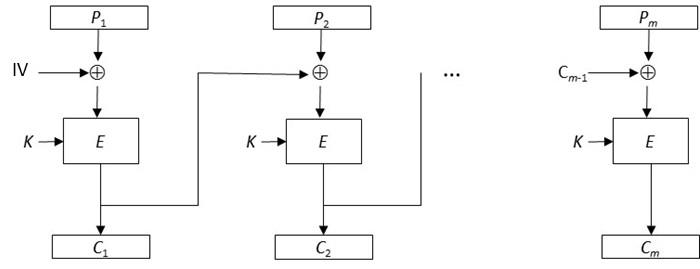
\includegraphics[width=0.85\textwidth]{../../images/python/page_030_img_01.jpeg}

\end{document}
